\documentclass[8pt,landscape,a4paper]{extarticle}
\usepackage{blindtext}
\usepackage[utf8]{inputenc}
\usepackage[nosf]{kpfonts}
\usepackage[default]{sourcesanspro}
\usepackage{multicol}
\usepackage{multirow}
\usepackage[top=3mm,bottom=4mm,left=2mm,right=3mm]{geometry}
\usepackage{wrapfig}
\usepackage{microtype}
\usepackage[framemethod=tikz]{mdframed}
\usepackage{enumitem}
\usepackage{amssymb}
\usepackage{scalerel}
\usepackage[explicit]{titlesec}
% \usepackage{hhline}
\usepackage{listings}   % to use nodes inside listing see: https://texample.net/tikz/examples/tikz-listings/ 
\usepackage{xcolor}
\usepackage{dirtytalk}
\usepackage[hidelinks,
            % set pdf metadata
            pdfauthor={Laurin Heitzer},
            pdftitle={ProgC++},
            pdfsubject={Programmieren in C++ FS23},
            pdfkeywords={Gahn go lerne!!}]{hyperref}
\usepackage{tabularx}
\usepackage{booktabs}
\usepackage{tikz-uml}   % for this to work, download tikz-uml.sty from https://perso.ensta-paris.fr/~kielbasi/tikzuml/index.php?lang=en to 'texlive/texmf-local/tex/latex/local' and run 'texhash' in ps terminal (windows)
\usepackage{realboxes}
\usepackage{tcolorbox}
\usepackage{textcomp}
\usepackage{pifont}

\usetikzlibrary{arrows, positioning,calc}
\usetikzlibrary{arrows.meta}
\usetikzlibrary{angles}
\usetikzlibrary{tikzmark}

\setlength{\columnsep}{1.5mm}           % space between columns
\setlength{\columnseprule}{0.1pt}       % vertical line between columns (set to 0 to remove)
\def\semester{FS23}                     % set Semester
\def\dozent{Prof.\ Dr.-Ing. C. Werner}  % set Dozent
\title{ProgC++}                         % set Title
\author{Laurin Heitzer}                 % set Author

\setcounter{secnumdepth}{0}
\definecolor{myblue}{cmyk}{1,.72,0,.38}
\definecolor{mygray}{cmyk}{0,0,0,.75}
\definecolor{cactgreen}{RGB}{100,190, 20}
\definecolor{redbg}{RGB}{235, 214, 214}
\definecolor{cbred}{RGB}{255, 0, 100}       % red for colorblind people (with more blue) see: https://davidmathlogic.com/colorblind/ 

% colors for listings (code)
\definecolor{codeblue}{RGB}{2, 90, 200}
\definecolor{codegreen}{rgb}{0,0.6,0}
\definecolor{codegray}{rgb}{0.5,0.5,0.5}
\definecolor{codepurple}{rgb}{0.58,0,0.82}
\definecolor{backcolour}{rgb}{0.95,0.95,0.92}

\setlength{\parindent}{0pt}                     % no indent at beginning of paragraph
\setlist[enumerate]{label*=-, leftmargin=*, }   % set default enumerate to - instead of 1. 2. 3. ...
\setlist[itemize]{label=-}   % set default itemize to -
\setlist{nosep}                                 % no space between items in lists

% change font size for super- and subscript
\catcode`_=\active
\catcode`^=\active

\newcommand_[1]{\ensuremath{\sb{\mathrm{\scaleobj{0.7}{#1}}}}}
\newcommand^[1]{\ensuremath{\sp{\mathrm{\scaleobj{0.7}{#1}}}}}

\def\subnode#1#2%
   {\tikz[remember picture,baseline=(#1.base),inner sep=0pt,
          outer sep=0pt,minimum width=0pt]\node(#1){#2};}

% custom inline tikz node
\newcommand{\tikznode}[2]{% from https://tex.stackexchange.com/a/402466/121799
	\ifmmode%
	\tikz[remember picture,baseline=(#1.base),inner sep=0pt] \node (#1) {$#2$};%
	\else
	\tikz[remember picture,baseline=(#1.base),inner sep=0pt] \node (#1) {#2};%
	\fi}


% custom inline tcolorbox
\newtcbox{\mybox}
            [1]
            [backcolour]
            {on line,
            arc=0pt,
            outer arc=0pt,
            colback=#1,
            colframe=#1,
            boxsep=0pt,
            left=1pt,
            right=1pt,
            top=1pt,
            bottom=1pt,
            boxrule=0pt}

\makeatletter

\newcommand{\bbr}[2]{\colorlet{saved}{.}\color{#1}\left(\color{saved}#2\color{#1}\right)\color{saved}}  % colored brackets
\newcommand{\cgn}[1]{{\color{lime}#1}}      % short command for lime text
\newcommand{\cct}[1]{{\color{cactgreen}#1}} % short command for cactgreen text
\newcommand{\abs}[1]{\left|#1\right|}       % short command for absolute markings
\newcommand{\real}{\mathbb{R}}              % short command for R (real numbers)
\newcommand{\limes}[1]{\underset{#1}{\lim}} % short command for limit with arrow below
\newcommand{\cmark}{{\color{cactgreen}\ding{51}}}   % cactgreen checkmark
\newcommand{\xmark}{{\color{cbred}\ding{55}}}       % red xmark

% custom inline listings with box around them
\newcommand{\mylstbox}[2][columns=fullflexible]{\mybox{\lstinline[#1]{#2}}}
\newcommand{\mytclstbox}[2][columns=fullflexible]{\mybox{\lstinline[basicstyle=\sffamily\footnotesize\color{#1}, columns=fullflexible]{#2}}}

\newcommand\addvmargin[1]{
  \node[fit=(current bounding box),inner ysep=#1,inner xsep=0]{};
}

\def\input@path{{./sections/}{./images/}{./tikz/}}
\graphicspath{{./images/}}

% custom title formats
\titleformat{\section}
            {\sffamily\normalsize\bfseries}
            {\thesection}
            {0mm}
            {\colorbox{lightgray!40}{\rule[-.2\baselineskip]{0pt}{2.5mm}\parbox{\dimexpr\columnwidth-2\fboxsep\relax}{\textcolor{myblue!40}{#1}}}}
\titlespacing{\section}
             {0mm}
             {.2ex}
             {.2ex}
% \renewcommand{\section}{\@startsection{section}{1}{0mm}%
%                                 {.2ex}%
%                                 {.2ex}%x
%                                 {\color{myblue}\sffamily\normalsize\bfseries}}
\renewcommand{\subsection}{\@startsection{subsection}{1}{0mm}%
                                {.2ex}%
                                {.2ex}%x
                                {\sffamily\normalsize\bfseries}}
\renewcommand{\subsubsection}{\@startsection{subsubsection}{1}{0mm}%
                                {.2ex}%
                                {.2ex}%x
                                {\color{mygray}\sffamily\normalsize\bfseries}}
\makeatother

% listings style (code)
\lstdefinestyle{mystyle}{
    backgroundcolor=\color{backcolour},   
    commentstyle=\color{codegreen},
    keywordstyle=\color{codeblue},
    numberstyle=\tiny\color{codegray},
    stringstyle=\color{codepurple},
    basicstyle=\sffamily\footnotesize,
    breakatwhitespace=false,         
    breaklines=true,                 
    captionpos=b,                    
    keepspaces=true,                 
    numbers=left,                    
    numbersep=2pt,                  
    showspaces=false,                
    showstringspaces=false,
    showtabs=false,                  
    tabsize=4,
	xleftmargin=1.2em,
	language=[11]C++,
	% frame=single,
	columns=[l]fullflexible	% see: https://tex.stackexchange.com/questions/99416/latex-source-code-listing-with-less-space-between-characters or manual
}

\lstset{
    style=mystyle,
    morekeywords={final, override}
    }

\newcommand{\mylstil}[1]{\lstinline[basicstyle=\sffamily\normalsize]{#1}}

% tikz-uml style
\tikzumlset{fill class=backcolour,font=\sffamily\footnotesize}

\begin{document}

% how to include code snippets: https://www.overleaf.com/learn/latex/Code_listing 

\begin{multicols*}{3}
	\vspace{-3mm}
\begin{center}
    \makeatletter
    \tikz[overlay, remember picture]{ \node[inner sep=0pt, outer sep=0pt] at (-0.7,-0.2) {\qrcode[level=L, version=0,height=0.9cm]{https://github.com/P4ntomime/ProgCPP}};}
    {\Large\bfseries \@title{} --- \semester{} --- \dozent{}}\\[3mm]
    {\large \@author}
    \makeatother
\end{center}\vspace{-1mm}

    
	% DONE: Klassen
    % DONE: add "best practices"
    % DONE: abstract methods "= 0;"-designator
	\section{Classes}
    \vspace{-2mm}
	\lstinputlisting{snippets/class.h}\vspace{-2mm}

\subsection{Styleguide}
    \mylstil{public}, \mylstil{protected} and \mylstil{private} members should be declared in that order.

\subsection{Best practices}
    \begin{enumerate}
        \item Default ctor; further ctors if needed
        \item Every user-defined ctor should initialize all member variables
        \item label user-defined dtor with \mylstil{virtual}
        \item "rule of zero" (if possible): no user-defined ctors, dtors, copy-ctors, move-ctors, copy-assignment-operators, move-assignment-operators
    \end{enumerate}

\subsection{Ctors}
    \begin{tabularx}{\columnwidth}{@{}l X@{}}
        \underline{Name:}          &Identical to class name\\
        \underline{Returntype:}    &None! Not void!\\
        \underline{Params:}        &Any\\
                            &-- none: default ctor\\
                            &-- const reference to own class: \textbf{copy-ctor}\\
        \underline{Task:}          &Prepares/initializes class
    \end{tabularx}

\subsection{Dtors}
    \begin{tabularx}{\columnwidth}{@{}l X@{}}
        \underline{Name:}          &Identical to class name\\
        \underline{Returntype:}    &None! Not void!\\
        \underline{Params:}        &None\\
        \underline{Task:}          &Deallocate memory/resources
    \end{tabularx}
    Only one destructor per class. (In some special cases overloading is possible)\newline
    Automatically called when class is no longer needed.
    
\subsection{Visibility}
    \begin{tabularx}{\columnwidth}{@{}l X@{}}
        \underline{Public:}       & Visible to everyone (within class, in derived, wherever class is used)\\
        \underline{Protected:}    & Only visible to class and derived classes\\
        \underline{Private:}      & Only visible within class
    \end{tabularx}
    
    \subsubsection{Friend attribute}
    A method within a class can be declared as \mylstil{friend}. Said method is then globally accessible and can access private members of the class.

    \subsubsection{Getter- and Setter-methods}
    Getter- and Setter-methods are used to control access to private members of a class. 
    They are public methods that return or set the value of a private member. 
    They can be used to check the validity of the value to be set or to hide the implementation of the class (e.g. if the class is part of a library).
    In certain cases the setter method can be declared as protected, if it is only to be used by the base- and derived classes.

    \subsection{UML (U\textcolor{gray}{nified} M\textcolor{gray}{odeling} L\textcolor{gray}{anguage})}
    \begin{center}
        \begin{tikzpicture}
    \umlclass[x=-2.7]{Super}{
        -privateMember: int\\
        \#protectedMember: char\\
        +publicMember: bool
    }{
        +publicMethod(): void\\
        \umlvirt{+publicVirtualMethod(parameter: int): void}\\
        \umlstatic{+staticMethod(): void}\\
        -privateMethod(): bool\\
        \#protectedMethod(value: int): char\\
        +Super()\\
    }
%     \node at (-1.75, 0.5) (pm) {};
%     \node at (-1.75, -0.4) (pmet) {};
%     \draw (pm) -- (-3.5,0.5) node[anchor=east] {Name} -- (pmet);
%     \node at (0.25, 0.5) (pmty) {};
%     \node at (1.8, -0.4) (pmetty) {};
%     \draw (pmty) -- (3.5,0.5) node[anchor=west] {(return)Type} -- (pmetty);
    \umlclass[x=2.5]{Derived}{
        +publicMember: bool
    }{
        +publicMethod(): void\\
        +Derived()\\
    }
    \umlinherit[geometry=--]{Derived}{Super}
\end{tikzpicture}
    \end{center}
    \vspace{-2mm}
    \mylstil{static} methods can be called without an instance of a class. They can be called like \mylstbox{Super.staticMethod();}. \mylstbox{+publicVirtualMethod()} refers to a \textit{pure virtual} method.
    
\subsection{Const}
    If \mylstil{const} is used after a method declaration, the method is not allowed to change any member variables of the class.

    \mylstbox{int someFunction() const;}

\subsection{Inheritance}
	If a class is to be inherited from, its destructor needs to be defined as virtual.
	A classic example of inheritance looks as follows:
    \vspace{-1mm}
	\lstinputlisting{snippets/inheritance.h}\vspace{-1mm}
	Classes can be derived from as \mylstil{public}, \mylstil{protected} or \mylstil{private}. Default of \mylstil{class} is \mylstil{private}, default of \mylstil{struct} is \mylstil{public}.
	This changes visibility of its inherited methods.
    \begin{center}
        \begin{tabular}{@{}l@{} c c@{}}
            \toprule
            \textbf{Inheritance visibility} & \textbf{visibility in base class} & \textbf{visibility in derived class}\\\toprule
            public (default w/ \mylstil{struct})   &\begin{tikzpicture}[baseline=-0.55cm, remember picture]
                                    \begin{scope}[every node/.style={fill=backcolour, minimum width=2cm, minimum height=0.45cm, align=center}]
                                        \node (box1pub) {public};
                                        \node[below=0.1mm of box1pub] (box1prot) {protected};
                                        \node[below=0.1mm of box1prot] (box1priv) {private};
                                    \end{scope}
                                    \addvmargin{0.5mm}
                                \end{tikzpicture}
                                &\begin{tikzpicture}[baseline=-0.55cm, remember picture]
                                    \begin{scope}[every node/.style={fill=backcolour, minimum width=2cm, minimum height=0.45cm, align=center}]
                                        \node (box2pub) {public};
                                        \node[below=0.1mm of box2pub] (box2prot) {protected};
                                        \node[below=0.1mm of box2prot] (box2priv) {invisible};
                                    \end{scope}
                                    \addvmargin{0.5mm}
                                \end{tikzpicture}\\\midrule
            protected           &\begin{tikzpicture}[baseline=-0.55cm, remember picture]
                                    \begin{scope}[every node/.style={fill=backcolour, minimum width=2cm, minimum height=0.45cm, align=center}]
                                        \node (box3pub) {public};
                                        \node[below=0.1mm of box3pub] (box3prot) {protected};
                                        \node[below=0.1mm of box3prot] (box3priv) {private};
                                    \end{scope}
                                    \addvmargin{0.5mm}
                                \end{tikzpicture}
                                &\begin{tikzpicture}[baseline=-0.55cm, remember picture]
                                    \begin{scope}[every node/.style={fill=backcolour, minimum width=2cm, minimum height=0.45cm, align=center}]
                                        \node (box4pub) {\color{gray!50}public};
                                        \node[below=0.1mm of box4pub] (box4prot) {protected};
                                        \node[below=0.1mm of box4prot] (box4priv) {invisible};
                                    \end{scope}
                                    \addvmargin{0.5mm}
                                \end{tikzpicture}\\\midrule
            private (default w/ \mylstil{class})          &\begin{tikzpicture}[baseline=-0.55cm, remember picture]
                                    \begin{scope}[every node/.style={fill=backcolour, minimum width=2cm, minimum height=0.45cm, align=center}]
                                        \node (box5pub) {public};
                                        \node[below=0.1mm of box5pub] (box5prot) {protected};
                                        \node[below=0.1mm of box5prot] (box5priv) {private};
                                    \end{scope}
                                    \addvmargin{0.5mm}
                                \end{tikzpicture}
                                &\begin{tikzpicture}[baseline=-0.55cm, remember picture]
                                    \begin{scope}[every node/.style={fill=backcolour, minimum width=2cm, minimum height=0.45cm, align=center}]
                                        \node (box6pub) {\color{gray!50}public};
                                        \node[below=0.1mm of box6pub] (box6prot) {\color{gray!50}protected};
                                        \node[below=0.1mm of box6prot] (box6priv) {\footnotesize private / invisibel};
                                    \end{scope}
                                    \addvmargin{0.5mm}
                                \end{tikzpicture}\\\bottomrule
        \end{tabular}
    \end{center}
    \begin{tikzpicture}[overlay, remember picture, >={Triangle[width=1.5mm, length=1.5mm]}]
        \draw[->] (box1pub.east) -- (box2pub.west);
        \draw[->] (box1prot.east) -- (box2prot.west);
        \draw[->] (box1priv.east) -- (box2priv.west);

        \draw[->] (box3pub.east) -- (box4prot.west);
        \draw[->] (box3prot.east) -- (box4prot.west);
        \draw[->] (box3priv.east) -- (box4priv.west);

        \draw[->] (box5pub.east) -- (box6priv.west) node[rotate=-27, midway, below=-1mm,xshift=-1mm] {\footnotesize private};
        \draw[->] (box5prot.east) -- (box6priv.west);
        \draw[->] (box5priv.east) -- (box6priv.west) node[midway, below=-0.5mm, xshift=-1mm] {\footnotesize invisible};
    \end{tikzpicture}\vspace{-2mm}
\subsubsection{ctor- and dtor-chaining}
    Order of ctor calls: base class(es) first, then derived class(es).\newline
    Order of dtor calls: derived class(es) first, then base class(es).\newline
    Example:
    \vspace{-2mm}
    \lstinputlisting{snippets/ctorchaining.cpp}\vspace{-2mm}
    Ctors are automatically chained, but can be explicitly called as well with an initializer list like in the example.

\subsubsection{vtable}
    \vspace{-2mm}
    \lstinputlisting{snippets/vtable.h}\vspace{-2mm}
    Previous code snippet of polymorphic code produces following memory map:
    \begin{center}
        % \begin{tikzpicture}
%     \umlclass[type=abstract]{Dog}{
%         -name_: string
%     }{
%         +Dog(name: string)\\
%         +\umlvirt{sit():void}\\
%         +\umlvirt{bark(): void}\\
%         +\umlvirt{getName(): void}
%     }
%     \umlclass[y=-2.5]{Husky}{

%     }{
%         +Husky(name: string)\\
%         +sit(): void\\
%         +bark(): void\\
%     }
%     \umlinherit[geometry=--]{Husky}{Dog}
%     \node[right=1.5cm of Dog, style={inner sep=0,outer sep=0}] (DogVtable) {%
%         \begin{tabular}{@{}c c@{}}
%             \toprule
%             {\bf\sffamily Method} &{\bf\sffamily Implementation}\\\toprule
%             {\sffamily sit()} &{\sffamily NULL}\\
%             {\sffamily bark()} &{\sffamily Dog::bark()}\\
%             {\sffamily getName()} &{\sffamily Dog::getName()}\\\bottomrule
%         \end{tabular}};
%     \draw[dashed, dash pattern=on 1mm off 1mm] (Dog) -- (DogVtable);
%     \node[right=1.5cm of Husky, style={inner sep=0,outer sep=0}] (HuskyVtable) {%
%         \begin{tabular}{@{}c c@{}}
%             \toprule
%             {\bf\sffamily Method} &{\bf\sffamily Implementation}\\\toprule
%             {\sffamily sit()} &{\sffamily Husky::sit()}\\
%             {\sffamily bark()} &{\sffamily Husky::bark()}\\
%             {\sffamily getName()} &{\sffamily Dog::getName()}\\\bottomrule
%         \end{tabular}};
%     \draw[dashed, dash pattern=on 1mm off 1mm] (Husky) -- (HuskyVtable);
% \end{tikzpicture}

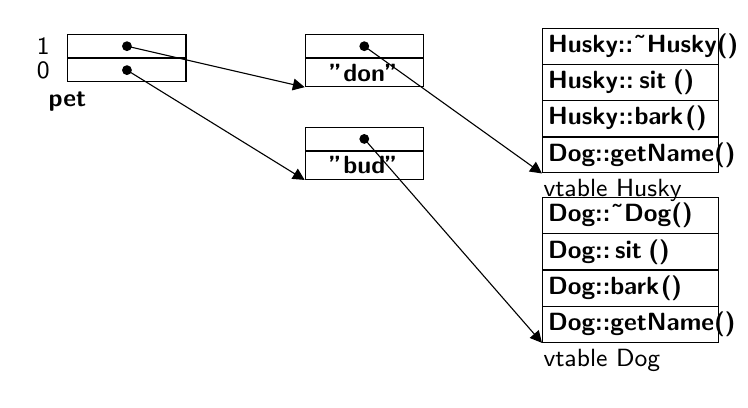
\begin{tikzpicture}[font=\sffamily\small]
    \node[draw, minimum width=1.5cm, minimum height=0.3cm] (petvt0) {};
    \node[draw, minimum width=1.5cm, minimum height=0.3cm, above=-0.1mm of petvt0] (petvt1) {};
    \node[left=1mm of petvt0] {0};
    \node[left=1mm of petvt1] {1};
    \node[below=0mm of petvt0.south west] {\bfseries pet};
    
    \node[draw, minimum width=1.5cm, minimum height=0.3cm, right=1.5cm of petvt1] (hskymm1) {};
    \node[draw, minimum width=1.5cm, minimum height=0.3cm, inner sep=0.7mm, anchor=west, below=-0.1mm of hskymm1] (hskymm0) {\bfseries "don"};
    
    \node[draw, minimum width=1.5cm, minimum height=0.3cm, below=0.5cm of hskymm0] (dogmm1) {};
    \node[draw, minimum width=1.5cm, minimum height=0.3cm, inner sep=0.7mm, anchor=west, below=-0.1mm of dogmm1] (dogmm0) {\bfseries "bud"};
    
    \node[draw, text width=2.1cm, minimum height=0.3cm, inner sep=0.7mm, anchor=west, right=1.5cm of hskymm1] (hskyvt3) {\lstinline[basicstyle=\sffamily\bfseries\small]{Husky::~Husky()}};
    \node[draw, text width=2.1cm, minimum height=0.3cm, inner sep=0.7mm, anchor=west, below=-0.1mm of hskyvt3] (hskyvt2) {\lstinline[basicstyle=\sffamily\bfseries\small]{Husky::sit()}};
    \node[draw, text width=2.1cm, minimum height=0.3cm, inner sep=0.7mm, anchor=west, below=-0.1mm of hskyvt2] (hskyvt1) {\lstinline[basicstyle=\sffamily\bfseries\small]{Husky::bark()}};
    \node[draw, text width=2.1cm, minimum height=0.3cm, inner sep=0.7mm, anchor=west, below=-0.1mm of hskyvt1] (hskyvt0) {\lstinline[basicstyle=\sffamily\bfseries\small]{Dog::getName()}};
    \node[rectangle, text width=2.1cm, minimum height=0.3cm, anchor=west, below=-0.5mm of hskyvt0, xshift=-0.5mm] {vtable Husky};
    
    \node[draw, text width=2.1cm, minimum height=0.3cm, inner sep=0.7mm, anchor=west, below=0.3cm of hskyvt0] (dogvt3) {\lstinline[basicstyle=\sffamily\bfseries\small]{Dog::~Dog()}};
    \node[draw, text width=2.1cm, minimum height=0.3cm, inner sep=0.7mm, anchor=west, below=-0.1mm of dogvt3] (dogvt2) {\lstinline[basicstyle=\sffamily\bfseries\small]{Dog::sit()}};
    \node[draw, text width=2.1cm, minimum height=0.3cm, inner sep=0.7mm, anchor=west, below=-0.1mm of dogvt2] (dogvt1) {\lstinline[basicstyle=\sffamily\bfseries\small]{Dog::bark()}};
    \node[draw, text width=2.1cm, minimum height=0.3cm, inner sep=0.7mm, anchor=west, below=-0.1mm of dogvt1] (dogvt0) {\lstinline[basicstyle=\sffamily\bfseries\small]{Dog::getName()}};
    \node[rectangle, text width=2.1cm, minimum height=0.3cm, anchor=west, below=-0.5mm of dogvt0, xshift=-0.5mm] {vtable Dog};

    \draw[-{Triangle[width=1.5mm, length=1.5mm]}] (petvt0.center) -- (dogmm0.south west);
    \draw[-{Triangle[width=1.5mm, length=1.5mm]}] (petvt1.center) -- (hskymm0.south west);
    \draw[-{Triangle[width=1.5mm, length=1.5mm]}] (dogmm1.center) -- (dogvt0.south west);
    \draw[-{Triangle[width=1.5mm, length=1.5mm]}] (hskymm1.center) -- (hskyvt0.south west);
    
    \node[circle, fill=black, minimum size=1.25mm, inner sep=0mm, outer sep=0mm] at (petvt0.center) {};
    \node[circle, fill=black, minimum size=1.25mm, inner sep=0mm, outer sep=0mm] at (petvt1.center) {};
    \node[circle, fill=black, minimum size=1.25mm, inner sep=0mm, outer sep=0mm] at (dogmm1.center) {};
    \node[circle, fill=black, minimum size=1.25mm, inner sep=0mm, outer sep=0mm] at (hskymm1.center) {};

\end{tikzpicture}
% \columnbreak
    \end{center}

\subsubsection{Redefinition of methods}
    Inherited methods can be redefined in derived classes. If said methods are declared as \textcolor{cactgreen}{\textbf{non-virtual}}, \textcolor{cactgreen}{\textbf{static binding}} is applied and it is determined at \textcolor{cactgreen}{\textbf{compile time}}, whether the base class' or the derived class' method is called. (depending on pointer or reference type)\newline
    If the method is declared as \textcolor{purple}{\textit{\textbf{virtual}}}, \textcolor{purple}{\textit{\textbf{dynamic binding}}} is applied at \textcolor{purple}{\textit{\textbf{runtime}}} and the derived class' method is called, even if the pointer or reference type is of the base class.

    Example:
    \vspace{-2mm}
    \lstinputlisting{snippets/polymorph.h}\vspace{-2mm}
    Classes that are declared as \textit{pure virtual} have no methods defined (method = 0) and cannot be instantiated. They can only be used as base classes for other classes. This is called an interface.

\subsection{Operator Overloading}
    Following operators can be overloaded:
    \vspace{-2mm}
    \lstinputlisting[numbers=none, backgroundcolor=\color{white}]{snippets/overloadable.h}\vspace{-2mm}
    Example:
    \vspace{-2mm}
    \lstinputlisting{snippets/classopov.h}\vspace{-2mm}
	
    
    % DONE: references
    \section{References}
    References are used like an alias to a variable. 

    With a variable \mylstbox{int var = 42;} a reference to it can be created with \mylstbox{int& myRef = var;}. 
    
    \mylstbox{myRef} can now be used exactly like \mylstbox{var}.
    
    References are never uninitialized and never have \mylstil{nullptr} as value.

    It is unspecified whether or not a reference requires storage.

\textbf{sizeof}: When using \mylstil{sizeof} on a reference, the size of the referenced object is returned.

\textbf{const}: By using \mylstil{const} on a reference, the referenced object cannot be changed.
    
	% DONE: function pointers
    \section{Function Pointers}
    \begin{tabular}{@{}l l@{}}
        Function:           &\mylstbox{int functionName(int a, int b);}\\
        Function pointer:   &\mylstbox{int (*functionPointer)(int, int);}
    \end{tabular}
    
    % DONE: (automatic) memory management (memory maps, vptr, vtable, maybe stack)
    % DONE: manual memory management (after delete null/nullptr), advantages/disadvantages
    \section{Memory management}
    \textbf{Automatic memory management}: done by compiler, located on stack, LIFO (last in, first out) data structure, stack pointer points to top of stack, grows downwards.

    \textbf{Manual memory management}: done by programmer, located on heap, order of allocation and deallocation not defined, heap grows upwards. After \mylstil{delete}/\mylstil{free()} pointer needs to be set to 0 / \mylstil{nullptr}.
    
    \section{Operators \& std libraries}\vspace{-2mm}
\begin{multicols*}{2}
    \begin{tabularx}{\columnwidth}{@{}l l@{}}
        \toprule
        \textbf{Operator} & \textbf{Example} \\
        \toprule
        \mylstbox{new} & \mylstbox{int* intPtr = new int;} \\
        \mylstbox{new[]} & \mylstbox{int* intArrPtr = new int[5];} \\
        \mylstbox{delete} & \mylstbox{delete intPtr;} \\
        \mylstbox{delete[]} & \mylstbox{delete[] intArrPtr;} \\
        \bottomrule
    \end{tabularx}
    \columnbreak%
    \begin{tabularx}{\columnwidth}{@{}l l@{}}
        \toprule
        \textbf{Library} & \textbf{Contents}\\
        \toprule
        \mylstbox{<iostream>} & \mylstbox{std::cin, std::cout, std::endl} \\
        \mylstbox{<string>} & \mylstbox{std::string} \\
        \mylstbox{<iomanip>} & \mylstbox{std::setw(), std::setfill()} \\
        \mylstbox{<fstream>} & \mylstbox{std::ifstream, std::ofstream} \\
        \bottomrule
    \end{tabularx}
\end{multicols*}\vspace{-2mm}
    
    \section{std formatting --- \textcolor{orange}{<iomanip>} \textcolor{blue}{<iostream>}}
\begin{tabularx}{\columnwidth}{@{}l l l@{}}
    \toprule
    \textbf{Flag} & \textbf{Description} &\textbf{Example}\\
    \toprule
    \mytclstbox[blue]{std::boolalpha}       & output bool as text               & \mylstbox[language=bash, keywordstyle=\color{black}]{true} or \mylstbox[language=bash, keywordstyle=\color{black}]{false}\\
    \mytclstbox[blue]{std::fixed}           & output as fixed point             & \mylstbox[language=bash]{3.141593}\\
    \mytclstbox[blue]{std::dec}             & output decimal                    & \mylstbox[language=bash]{42}\\
    \mytclstbox[blue]{std::hex}             & output hexadecimal                & \mylstbox[language=bash]{2a}\\
    \mytclstbox[blue]{std::oct}             & output octal                      & \mylstbox[language=bash]{52}\\
    \mytclstbox[orange]{std::setprecision(6)} & set precision of next output      & \mylstbox[language=bash]{3.14159}\\
    \mytclstbox[orange]{std::setw()}          & set width of next output          & \textit{see below}\\
    \mytclstbox[orange]{std::setfill()}       & set fill character                & \mylstbox[language=bash]{*******-1.23}\\
    \mytclstbox[blue]{std::internal}        & fill between sign and digits      & \mylstbox[language=bash]{-*******1.23}\\
    \mytclstbox[blue]{std::left}            & fill on the right                 & \mylstbox[language=bash]{*******-1.23}\\
    \mytclstbox[blue]{std::right}           & fill on the left                  & \mylstbox[language=bash]{-1.23*******}\\
    \mytclstbox[blue]{std::scientific}      & output as scientific notation     & \mylstbox[language=bash]{3.141593e+00}\\
    \mytclstbox[orange]{std::showbase}        & show base of numbers              & \mylstbox[language=bash]{0x2a}\\
    \mytclstbox[orange]{std::showpoint}       & show decimal point                & \mylstbox[language=bash]{3.}\\
    \mytclstbox[orange]{std::showpos}         & show sign of positive numbers     & \mylstbox[language=bash]{+42}\\
    \mytclstbox[orange]{std::skipws}          & skip whitespace                   & \\
    \mytclstbox[orange]{std::unitbuf}         & flush after each output           & \\
    \mytclstbox[orange]{std::uppercase}       & use uppercase for hex \& float    & \mylstbox[language=bash]{2A}\\
    \mytclstbox[orange]{std::nouppercase}     & use lowercase for hex \& float    & \mylstbox[language=bash]{2a}\\
    \bottomrule
\end{tabularx}
	
    % DONE: order of declaration in .h and .cpp
    \section{Styleguide}
\begin{tabularx}{\columnwidth}{@{}l l@{}}
    \toprule
    \textbf{.h}                                 & \textbf{.cpp} \\
    \toprule
    include guard \mylstbox{#pragma once}       & header-comment \\
    header-comment                              & include own headers "\ldots"\\
    include system libraries <\ldots>           & include system libraries <\ldots>\\
    include projectspecific libraries "\ldots"  & include projectspecific libraries "\ldots"\\
    definition of constants                     & global / static variables\\
    typedefs, structs, classes                  & preprocessor directives\\
    extern-declaration of global variables      & function prototypes\\
    function prototypes                         & function / class definitions\\
                                                \bottomrule
\end{tabularx}

	% DONE: Compiler args.
    \section{Compiler Arguments}
    Compiling with clang++: \mylstbox[language=bash]{clang++ -Wall -o main main.cpp}

    With multiple source files: \mylstbox[language=bash]{clang++ -Wall -o main main.cpp other.cpp}

    Following are the most commonly used compiler arguments for clang++:
    
    \begin{tabular}{@{}l l@{}}
        -Wall & Enable all warnings \\
        -o & Output file \\
        -c & Compile to object file (mainly used in makefiles)\\
        -std=c++11 & Use C++11 standard
    \end{tabular}
    
    
	% DONE: Makefiles
    \section{Makefiles}
    Used to automate compilation process. Useful when working with multiple source files. \texttt{make} checks which files have changed and only compiles those (timestamps).\vspace{-1mm}
    \lstinputlisting[language=make, keywordstyle=\color{black}, escapechar=!]{snippets/Makefile}\vspace{-2mm}
    
    \begin{tikzpicture}[remember picture, overlay, >={Triangle[width=1.5mm, length=1.5mm]}]
        \node [right = 2cm of depend, text width=3cm] (deptext) {\sffamily Dependencies};
        \node [above = -1.5mm of deptext, text width=3cm] (tgttext) {\sffamily Target};
        \node [below = 6mm of deptext, text width=3cm] (tabtext) {\sffamily Tab (very important)};

        \draw[->, rounded corners=2pt] (tgttext) -| (target.north);
        \draw[->, rounded corners=2pt] (deptext) -- (depend);
        \draw[->, rounded corners=2pt] (tabtext) -| (indent.south);
    \end{tikzpicture}
    \begin{tabular}{@{}l l@{}}
        .PHONY: &Targets that do not produce an output are called \say{phony targets}.\\
        \$@ &Filename of target\\
        \$\textless{} &Filename of first dependency\\
        \$\textasciicircum{} &List of all dependencies\\
    \end{tabular}
    
    
    % DONE: assertions
    \section{Assertions}
    Assertions are used in testing to check if a condition is true. If the condition is false, the program will terminate with an error message.
    
    Found in \mylstbox{<cassert>} \qquad Usage: \mylstbox{assert(condition);}
    
	% DONE: templates
    \section{Templates}
\subsection{Function templates}
Function declaration:
\vspace{-2mm}
\lstinputlisting{snippets/funtemplate1.h}\vspace{-2mm}

Function definition:
\vspace{-2mm}
\lstinputlisting{snippets/funtemplate2.h}\vspace{-2mm}
Function templates can be used as \mylstbox{functionName<type1, type2,...>(param1, param2,...);} or \mylstbox{functionName(param1, param2, ...);}. The compiler will deduce the types of the template parameters from the function arguments.

\subsection{Class templates}
Class declaration:
\vspace{-2mm}
\lstinputlisting{snippets/classtemplate1.h}\vspace{-2mm}
Class definition:
\vspace{-2mm}
\lstinputlisting{snippets/classtemplate2.h}\vspace{-2mm}
Class templates can be used as \mylstbox{className<type1, type2,...> objectName;}. The compiler will deduce the types of the template parameters from the object declaration.

\subsection{Rules}
\begin{enumerate}
    \item Templates are \textbf{always} evaluated at \textbf{compile time}.
    \item To instantiate a template, the compiler needs to know following three things:
    \begin{enumerate}
        \item[1.] The template declaration
        \item[2.] The template definition
        \item[3.] Values for the template parameters
    \end{enumerate}
    \item Definition of template functions and methods need to be in the same file as the declaration (.h).
\end{enumerate}
    
	% DONE: typecasting (c++ style)
    \section{Typecasting}
    \textcolor{teal}{Implicit} typecasting is allowed in following cases:
    \begin{enumerate}
        \item Between \textcolor{teal}{all numerical types} (including bool)
        \item Between \textcolor{teal}{\textbf{some} pointer types} (complicated ruels)
        \item Instances of a subclass can be implicitly assigned to a variable of the superclass type \mylstbox{SuperClass s = SubClass();}
    \end{enumerate}
    \textcolor{violet}{Explicit} typecasting allows following operators:\vspace{1mm}\\
    \mylstbox[basicstyle=\sffamily\small]{static_cast<newType>(value of oldType)}: (most common)
    \begin{enumerate}
        \item Can cast pointer- and reference-types to instances of super- and subclasses in both directions.
        \item Can be used for all implicit casts.
        \item No typechecking at runtime.
    \end{enumerate}
    \mylstbox[basicstyle=\sffamily\small]{dynamic_cast<newType>(value of oldType)}: (for polymorphic types)
    \begin{enumerate}
        \item Can cast pointer- and reference-types to instances of polymorphic super- and subclasses in both directions.
        \item Checks at runtime (with RTTI) if the cast is valid. Returns \mylstil{nullptr} if invalid.
        \item Can cast pointer- and reference-types of non-polymorphic subclasses to superclasses (up-casting), but not the other way round (down-casting).
    \end{enumerate}
    \mylstbox[basicstyle=\sffamily\small]{const_cast<const type>(value of type)}: (only special cases)
    \begin{enumerate}
        \item Able to cast away const-ness or volatile-ness of a pointer or reference and the other way round.
    \end{enumerate}
    \mylstbox[basicstyle=\sffamily\small]{reinterpret_cast<newType>(value of oldType)}: (only special cases)
    \begin{enumerate}
        \item Can cast pointer- and reference-types to any other pointer- and reference-types.
        \item No typechecking at runtime.
        \item Reinterprets the bits of the oldType as the newType.
        \item \mylstbox{reinterpret_cast} is platform dependent and should be avoided.
    \end{enumerate}

\begingroup
\renewcommand{\arraystretch}{0.8}
    \begin{tabularx}{\columnwidth}{@{}l c l l c@{}}
        \toprule
        \textbf{Previous type}  &               & \textbf{New type}         & \textbf{Cast-type}                    &\textbf{Implicit}\\
        \toprule
        \mylstbox{float}        & $\rightarrow$ & \mylstbox{double}         & \mylstbox{static_cast}                & \cmark\\
        \mylstbox{int*}         & $\rightarrow$ & \mylstbox{unsigned int*}  & \mylstbox{reinterpret_cast}           & \xmark\\
        \mylstbox{const Animal} & $\rightarrow$ & \mylstbox{Animal}         & no cast                               & \cmark\\
        \mylstbox{Animal*}      & $\rightarrow$ & \mylstbox{Bird*}          & \mylstbox{dynamic_cast}               & \xmark\\
        \mylstbox{int}          & $\rightarrow$ & \mylstbox{float}          & \mylstbox{static_cast}                & \cmark\\
        \mylstbox{Bird*}        & $\rightarrow$ & \mylstbox{int*}           & \mylstbox{reinterpret_cast}           & \xmark\\
        \mylstbox{int}          & $\rightarrow$ & \mylstbox{bool}           & \mylstbox{static_cast}                & \cmark\\
        \mylstbox{volatile int*}& $\rightarrow$ & \mylstbox{volatile short*}& \mylstbox{reinterpret_cast}           & \xmark\\
        \mylstbox{Bird}         & $\rightarrow$ & \mylstbox{Animal}         & \mylstbox{static_cast}                & \cmark\\
        \mylstbox{volatile int*}& $\rightarrow$ & \mylstbox{int*}           & \mylstbox{const_cast}                 & \xmark\\
        \mylstbox{Bird*}        & $\rightarrow$ & \mylstbox{Animal*}        & \mylstbox{static_cast / dynamic_cast} & \cmark\\
        \mylstbox{int&}         & $\rightarrow$ & \mylstbox{short&}         & \mylstbox{reinterpret_cast}           & \xmark\\
        \bottomrule
    \end{tabularx}
\endgroup
    
	% DONE: exceptions
    \section{Exceptions}
    Exceptions are thrown using the \mylstil{throw} keyword. Usually this is within a \mylstil{try...catch} block or a function within such a block.
\vspace{-2mm}
\lstinputlisting{snippets/except1.cpp}\vspace{-4mm}
\hskip 0.2\columnwidth\rule[0mm]{0.6\columnwidth}{0.1pt}
\vspace{-2mm}
\lstinputlisting{snippets/except2.cpp}\vspace{-2mm}
    If an error is thrown without a \mylstil{try...catch} block, \mylstbox{std::terminate()} is called, which ends the program.
    The behaviour of this can be changed by setting a user-defined \mylstbox{std::terminate_handler} using \mylstbox{std::set_terminate()}.
    
    Functions and methods that don't throw exceptions should be marked with the \mylstil{noexcept} keyword. Otherwise \mylstil{noexcept(false)} can be used to mark a function that can throw exceptions.
    \mylstbox{std::exception} can be found within \mylstbox{<stdexcept>}.

\end{multicols*}

\end{document}